\documentclass[a4paper,12pt]{report}
\usepackage{fancyhdr}
\fancyhead[L]{}
\fancyhead[C]{2020.07.17 Főmérnöki utasítás}
\fancyhead[R]{}
\fancyfoot[L,R]{}
\fancyfoot[C]{\thepage}
\renewcommand{\headrulewidth}{0.4pt}
\renewcommand{\footrulewidth}{0.4pt}


\usepackage{geometry}
\newgeometry{textwidth=16cm}
\usepackage{amsfonts}
\usepackage{amssymb}
\usepackage[T1]{fontenc}
\usepackage[utf8]{inputenc}
\PassOptionsToPackage{defaults=hu-min}{magyar.ldf}
\usepackage[magyar]{babel}
\setcounter{secnumdepth}{5}
\usepackage{graphicx}
\usepackage{multirow}
\usepackage{nowidow}[all]
\usepackage{pdfpages}


\newcommand{\mksz}{Motoros Könnyűrepülő Szövetség\ }

\title{%
    \textbf{\mksz\\FŐMÉRNÖKI UTASÍTÁS}
}


\author{}
\date{2020.10.17.}

\begin{document}

\maketitle
\pagestyle{fancy}

\section*{Az utasítás célja}
Motoros sárkányrepülő eszközök üzembiztonságának növelés, repülés közben kialkuló veszélyes helyzetek kialakulásának csökkentése.
\\

\textbf{
A soron következő első repülés előtt a pilótának végre kell hajtani a flatterzsinórók bekötésének ellenőrzést. Az ellenőrzés tényét az üzemi naplóban dokumentálni kell!
\textit{,,Latnizsinórok bekötése ellenőrizve, a bekötések állapota megfelelő.''}
}
\\

\noindent
\textbf{Az ellenőrzés módja:} szemrevételezés, terheléspróba. \\A terheléspróbához a flatterzsinórt a kötélszívnél, a szárnyat a bekötő hevedernél megfogva és ellentartva a zsinórt meg kell húzni. Szemrevételezéssel ellenőrzni kell a heveder és a szárnyhoz történő rögzítés épséget. A hevederen és a heveder bekötésén szakadás, rojtosodás nem megengedett.

\section*{Az utasítás kategóriája}
\begin{center}
\textbf{JAVASLAT}
\end{center}

A repülő eszköz tulajdonosának, üzembentartójának saját belátása szerint kell végrehajtani az utasításban foglatakat! 

\section*{Érintett repülő eszközök}
Az utasításban érintettek a flatterzsinórókkal rendelkező motoros sárkányrepülőgép szárnyak.

Az állandaón összeszerelt repülő eszközök esetén a flatterzsinórok és bekötésük ellenőrzése csak pódiumról, létráról ellenőrizhető. A tárolás módjától függően a napsugárzás hatására, -- vagy rágcsálók megrágják --, a heveder roncsolódhat, elszakadhat.

A szárny minden szét- és összeszerelése közben a zsinórók meghúzásával meg kell győzödni a rögzítő hevederek teherviselő képességéről.

A flatterzsinórok \aref{flatter1}. ábrán látható rögzítése esetén a piros körrel jelölt heveder szakadása esetén a sodrony elszabadul, és a légcsavar síkjába kerülhet.

A szabad zsinór roncsolhatja a lágcsavart, vagy arra feltekerdve a szárny további jelentős sérülését okozhatja.

\section*{Megoldás}
A flatterzsinór eredeti rögzítését biztosító heveder szakadása esetén egy kiegészítő zsinór a sodronyt nem engedi elmozdulni, így az nem kerülhet a légcsavarkörbe.

A sodrony kötélszívén keresztül egy kiegészítő, zsinórt kell átvezetni és a latnizsinór köré hurkolva megcsomózni. A kiegészító zsinóroknak kellően lazáknak kell lenniük, ahhoz, hogy ne vegyék át az eredeti bekötések tartó szerepét.

A kiegésztő zsinór anyaga lehet \textit{paracord}, a latnizsinór anyagával megegyező, fonatolt (körszövött) műanyag (PP - polipropilén) alapú, 2-4\,mm vastag kötél.
A kötélnek teherhordó szerepe nincs, az eredeti rögzítés szakadása esetén a
flatterzsinórra ható légerőknek kell ellenállnia.

A kiegészítő kötél nem kerülhet a karabíner alá! Erre a szárny összeszerelésekor külön figyelmet kell fordítnai!

\Aref{flatter2}. ábrán látható a szárny középső részén kialakított flatterzsinór kiegészítő kötél elvezetése. 

\section*{Súlyponthelyzet}
A kiegészítő kötél nem változtatja meg a szárny repülési tulajdonságait, a a súlypont helyzetére nincs hatással.



\begin{figure}[ht!]
\centering
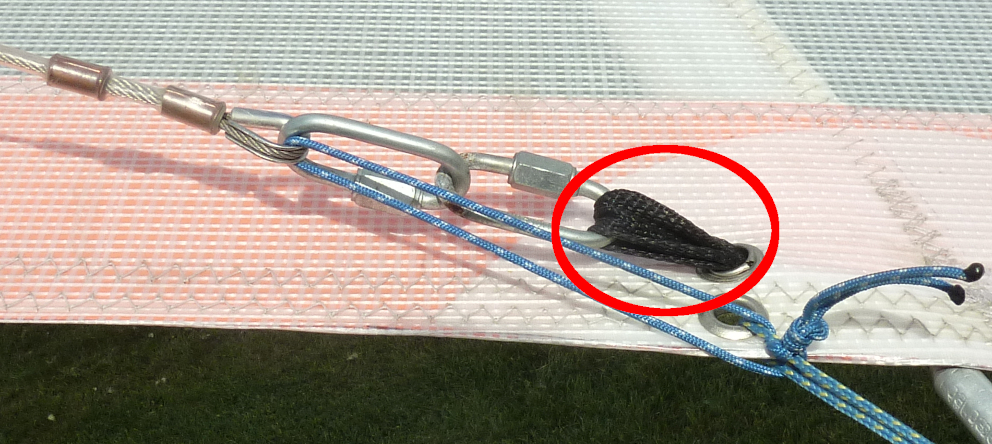
\includegraphics{kepek/1.jpg}
\caption{Flatter zsinór rögzítés}\label{flatter1}
\end{figure}

\begin{figure}[ht!]
\centering
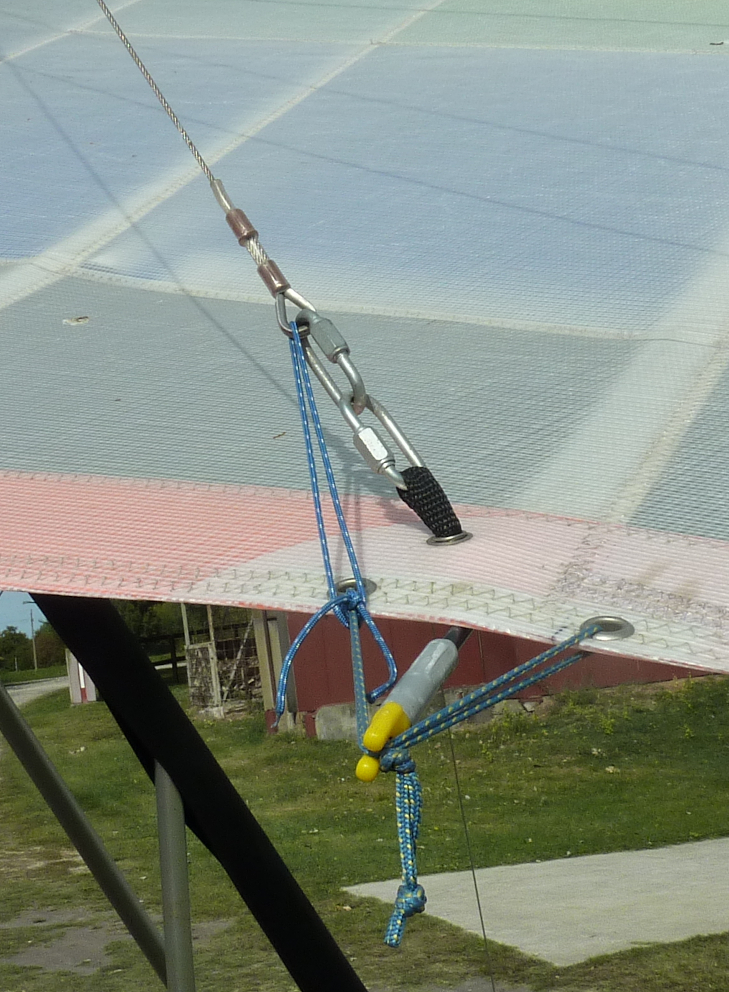
\includegraphics{kepek/2.jpg}
\caption{Flatter zsinór rögzítés szárnyközépen}\label{flatter2}
\end{figure}




%
%%
%%%
%%
% 
\end{document}
